%!TEX root = ../Dissertation.tex

\section{The Inexact Epigraphical Cutting Plane Algorithm}

% \begin{figure}

% \noindent\rule[0.1ex]{1\columnwidth}{0.5pt}
% {Inexact Epigraphical Cutting Plane}
 
% \vspace{-2mm}
% \noindent\rule[0.1ex]{1\columnwidth}{0.5pt}

% %\begin{algorithm}
% % \State $P_0 = C \times {[\mbox{upper bound on $f$}, \mbox{lower bound on $f$}]}$
% % \While {$\max\{ \mbox{height}(P_k), K \cdot \mbox{size}(P_k)^{1/(n+1)} \} \geq \mbox{TOL}$}
% %   \State $(t_k,x_k) \gets \mbox{\bf center}(P_k)$
% %   \State $\epsilon_k \gets \gamma (\min \{ u_0, \dots, u_{k-1}\}-t_k )$
% %   \State $(u_k,l_k,g_k)\gets F(x_k, \epsilon_k )$
% %   \State $P_{k+1}\gets P_k\cap 
% %       \underbrace{\{(t,x)\mid t\leq u_k \}}_{\mbox{\tiny upper bound}} \cap 
% %       \underbrace{\{(t,x)\mid l_k+g_k^{T}(x-x_k)\leq t\}}_{\mbox{\tiny lower bound}}$
% %   \vspace{-4mm}
% %   \State $k \gets k+1$  
% % \EndWhile
% %\end{algorithm}
% \noindent\rule[0.1ex]{1\columnwidth}{0.5pt}
% \caption{MVE Epigraphical Cutting Plane Algorithm. $K$ is constant which depends on the $\mbox{\bf center}$, and $\mbox{size}$ is a function which takes convex 
% sets into real values, depending on $\mbox{\bf center}$. } \label{alg:cutting_plane_epi_err}
% \end{figure}

Our proposed algorithm is a modification of the cutting plane algorithms
described in Section [] to accomidate
\begin{algorithm} 
  \SetKwInOut{Input}{input}\SetKwInOut{Output}{output}
  \SetKwProg{Fn}{function}{}{end}
  \SetAlgoNoLine
  \DontPrintSemicolon
  $P_0 = C \times {[\mbox{upper bound on $f$}, \mbox{lower bound on $f$}]}$\;
  
  \While {$\max\{ \mbox{height}(P_k), K \cdot \mbox{size}(P_k)^{1/(n+1)} \} \geq \mbox{TOL}$} {
  \nl $(t_k,x_k) \gets \mbox{\bf center}(P_k)$\;
  \nl $\epsilon_k \gets \gamma (\min \{ u_0, \dots, u_{k-1}\}-t_k )$\;
  \nl $(u_k,l_k,g_k)\gets F(x_k, \epsilon_k )$\;
  \nl $P_{k+1}\gets P_k\cap 
      \underbrace{\{(t,x)\mid t\leq u_k \}}_{\mbox{\tiny upper bound}} \cap 
      \underbrace{\{(t,x)\mid l_k+g_k^{T}(x-x_k)\leq t\}}_{\mbox{\tiny lower bound}}$\;
  \vspace{-5mm}
  \nl $k \gets k+1$  
  }
  \caption{Epigraphical Cutting Plane With Error \label{alg:cutting_plane_epi_err}}
\end{algorithm}
\noindent We will two consider methods of determining $\mbox{\bf center}$, the
center of gravity and the center of the maximum inscribed ellipsoid. In this
section, we will refer to the height of a convex set to be:
$$
\mbox{\rm height}(P)=\max\{t\mid(t,x)\in P\}-\min\{t\mid(t,x)\in P\}.
$$
We will refer to $u^*_k$ as the best upper bound and $l^*_k$ to be the strongest lower bounds.
\[
u^*_k = \min{ \{ u_0, \dots, u_{k-1}\} } \qquad l^*_k(x) = \max_{i < k}\{l_i + g_i^T(x-x_i)\}.
\]
There is an important property of the localization polytopes $P_k$ our method will exploit. Every polytope $P_k$ can be decomposed into the intersection of two sets,
one formed by the intersection of all the lower bounds, other a halfspace
formed by the intersection of the upper bounds, i.e.
$$
P_k = \mbox{epi}(l^*_k) \cap \{(t,x) \mid t \leq u^*_k\}
$$
The level sets of an epigraph are nested, and $\{x \mid (t,x) \in P_k\} $ is the level set of $l^*$ lower bound at $t$,
\[
t_1 \leq t_2 \Rightarrow \{x \mid (t_1,x) \in P_k\} \subseteq \{x \mid (t_2,x) \in P_k\}
\]
and thus every vertical half line emanating from inside the polytope will
only exit the polytope at the upper bound. We will refer to this as $P_k$ tapering downwards.


% $$
% \frac{u_0-f(x^*)}{\volmu(\mbox{conv}\{u_0\times\mbox{lvl}(f,u_0),(f(x^*),x^*)\})^{1/(n+1)}}.
% $$

% \noindent\rule[0.5ex]{1\columnwidth}{0.5pt}
% \begin{enumerate}
%   \item $P_0\supseteq\mbox{epi}(f)$
%   \item While $\max\{ \mbox{height}(P_k), K\volmu(P_k)^{1/(n+1)} \} \geq\epsilon$
%   \begin{enumerate}
% %   \item $\mathcal{E}_k=\mbox{maximum inscribed ellipse of }P_k$
%     \item $(t_k,x_k) = \mbox{\bf center}(P_k)$
%     \item $(u_k,l_k,g_k)=F(x_k,\tfrac{1}{50}(t_k - u_{k-1}))$
%     \item $P_{k+1}=P_k\cap 
%       \underbrace{\{(t,x)\mid t\leq u_k \}}_{\mbox{\tiny lower bound}} \cap 
%       \underbrace{\{(t,x)\mid l_k+g_k^{T}(x-x_k)\leq0\}}_{\tiny \mbox{upper bound}}$
% \end{enumerate}
% \end{enumerate}
% \vspace{1mm}
% \noindent\rule[0.5ex]{1\columnwidth}{0.5pt}

\subsection{The Center of Gravity Oracle} 

We begin our exposition with a conceptual algorithm. For this section
only, define
$$
\mbox{\bf center}(P) := \mbox{center of gravity of $P$} = \frac{\int_P z dz}{\int_P dz} \quad \mbox{and} \quad \mbox{size}(P) = \vol(P).
$$
This definition is valid when $P$ is bounded and has a nonempty interior,
which is true for all localization polyopes. The following theorem establishes
an important geometric fact about the CG.

\begin{thm} {\bf (Grunbaum's Theorem)} \label{thm:CG_cut} 
Let $a$ be the center of gravity of $P$. Then for any $g$,
$$
 \frac{1}{\exp(1)} \leq \frac{\vol(P \cap \{ x \mid g^T(x - a)\leq 0\}) }{\vol(P)} \leq 1- \frac{1}{\exp(1)} 
$$
\end{thm}

The center of gravity can therefore be interpreted as a $n$ dimensional analog
of a midpoint, as it divides a convex set into two approximately equal parts.

\begin{lem}\label{Rate-Decrease_cg}
The volumes decrease at the rate
\[
\frac{\vol(P_{k+1})}{\vol(P_k)}\leq  1-\frac{1-\gamma}{\exp(1)}
\]
\end{lem}
\begin{proof}

\noindent\textbf{Case 1: (Deep Cut) $l_k \geq t_k$ or $l_k \leq t_k$ and $u_k \leq t_k$ } 
The intersection of the cutting planes do not contain $(t_k,x_k)$, therefore by Theorem \ref{thm:MIE_cut},
\[
\frac{\vol(P_{k+1})}{\vol(P_k)}\leq 1 - \frac{1}{\exp(1)}
\]
\textbf{Case 2: (Shallow Cut) $l_k < t_k$ and $u_k > t_k$}. 
See Figure \ref{fig:shallow-cut} for an illustration of this case. 
By the definition of $\epsilon$,
\[
u_k-t_k \leq u_k-l_k\leq \gamma(u^*_k - t_k) \quad \Rightarrow \quad t_k + \gamma(u^*_k - t_k) \geq u_k 
\]
Define $\bar{P}_k$ to be the region above the upper cutting plane, compressed 
by a small amount from the top
\begin{align*}
\bar{P}_k & = \Sigma \big(P_{k}\cap\{(t,x)\mid t\geq t_{k}\} - (u^*_k, 0, \dots, 0) \big) + (u^*_k, 0, \dots, 0) \\
\Sigma & =\mbox{diag}(1-\gamma,1,\dots,1)
\end{align*}
The bottommost point of $\bar{P}_k$ is $(t_k+\gamma(u^*_k-t_k), x_k)$ which lies above $u_k$. Furthermore because the set tapers downwards, so $P_{k}\cap\{(t,x)\mid t\geq u_{k}\} \supseteq \bar{P}_k $. Therefore, taking volumes on both sides
\begin{equation} \label{eq:vol-ineqaality-compression}
\vol(P_k\cap\{(t,x)\mid t\geq u_{k}\})\geq (1-\gamma) \cdot \vol(P_k\cap\{(t,x)\mid t\geq t_{k}\})
\end{equation} 
Now
\begin{align*}
\vol(P_{k+1}) 
 & \overset{(a)}{\leq} \vol(P_k)-\vol(P_k\cap\{(t,x)\mid t\geq u_k\})\\
 & \overset{(b)}{\leq}\vol(P_k)-(1-\gamma)\cdot\vol(P_k\cap\{(t,x)\mid t\geq t_k\})\\
 & \overset{(c)}{\leq}\vol(P_k)-(1-\gamma) e^{-1}\cdot\vol(P_k) 
 = (1 - (1-\gamma)e^{-1} )\cdot \vol(P_k)
\end{align*}
$(a)$ comes from the fact that $P_{k+1}$ is $P_k$ intersected with two cutting planes. The right hand side of $(a)$ is the volume of $P_k$ intersected with just the upper bound. $(b)$ comes from \eqref{eq:vol-ineqaality-compression}. $(c)$ comes from Theorem \ref{thm:CG_cut}. Combing the two results, we obtain the theorem. 
\end{proof}

\begin{figure}
\begin{centering}
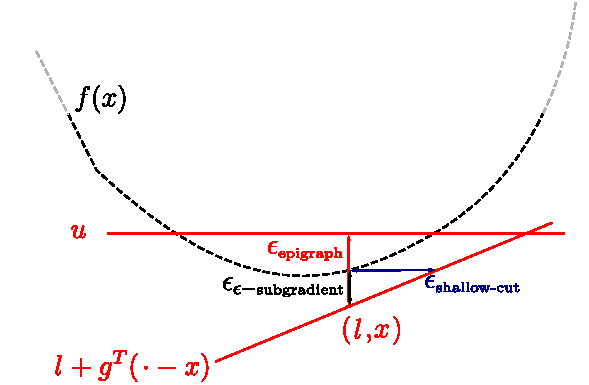
\includegraphics[width=0.65\textwidth]{cutting/fig0.pdf}
\par\end{centering}
\caption{Illustration of a shallow cut with an inexact epigraphical oracle. The dotted
line is $f(x)$, the polytope defined by the black solid lines $P_k$. The black
dot is center, and the two red lines are the two cutting planes provided by the 
oracle. \label{fig:shallow-cut}} 
\end{figure}

% \begin{lem} \label{lem:cg_non_strongly_convex_convergencegenc}
% Let $\mathcal{K}_0$ be the cone formed by the level set of $f$ at $u_0$ and the 
% optimal solution, 
% $$\mathcal{K}_{0}=\mbox{{\rm conv}}\{\sup_{x\in S}f(x)\times S,(f(x^{*}),x^{*})\}.$$
% Then for all $k$
% \[
% u^*_{k}-f(x^*)\leq K \cdot \vol(P_{k})^{1/(n+1)}, \qquad K := \frac{u_0-f(x^*)}{\vol(\mathcal{K}_0)^{1/(n+1)}}
% \]
% \end{lem}

% \begin{proof}
% Let $\mathcal{K}_k =\mathcal{K}_0\cap\{(t,x)\mid t \leq u^*_k\}$. Then 
% \[
%   \vol(P_k)\overset{(a)}{\geq}\vol(\mathcal{K}_k)\overset{(b)}{=}
%   \left(\frac{u^*_k-f(x^*)}{u_0-f(x^*)}\right)^{n+1} \!\!\!\!\!\!\cdot \vol(\mathcal{K}_0)
% \]
% $(a)$ comes from the fact that $P_k\supseteq\mathcal{K}_k$. $(b)$ comes from the fact
% that $\mathcal{K}_k$ is just $\mathcal{K}_0$ scaled about the
% base. Taking powers of $1/(n+1)$ on both sides, we get the desired result.
% \end{proof}

Combining the above result with Lemma \ref{lem:non_strongly_convex_convergencegen}, we get a final theorem on the convergence rate of our algorithm.
\begin{thm}\label{thm:MIE-convergence}
For all $k$
\[
u_{k}^{*}-f(x^{*})\leq K\left(1-\frac{1-\gamma}{\exp(1)}\right)^{k/(n+1)}\quad K=(u_{0}-f(x^{*}))\left(\frac{\vol(P_{0})}{\vol(\mathcal{K})}\right)^{1/(n+1)}
\]
and when 
Algorithm \ref{alg:cutting_plane_epi_err} with $\mbox{\bf center}$ being the
center of gravity terminates in no more than
\[
k = \left\lceil \frac{(n+1)\log(K/\mbox{TOL})}{-\log(1-(1-\gamma)/\exp(1))} \right\rceil 
\in \mathcal{O}\left(n\log\frac{1}{\mbox{TOL}}\right).
\]

\end{thm} 

We now focus our attention on the amount of work involved in each
oracle call. Recall that the cost of invoking the oracle is inversely
proportional to $\epsilon_k$. Hence we will show a lower bound on $\epsilon_k$
in the next few lemmas.


\begin{figure}
\begin{centering}
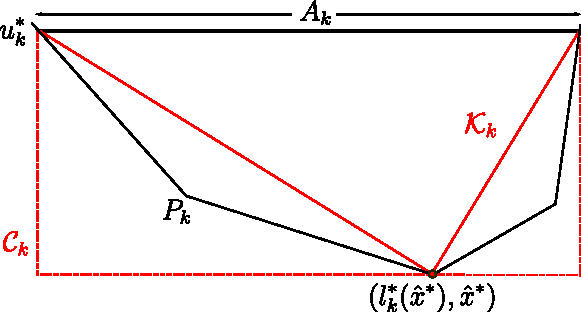
\includegraphics[width=0.65\textwidth]{cutting/fig6.pdf}
\par\end{centering}
\caption{Illustration of outer cylindrical approximation $\mathcal{C}_k$ and inner conic approximation $\mathcal{K}_k$ of $\mathcal{P}_k$} \label{fig:outer-inner-approx}
\end{figure} 

\begin{lem}\label{lem:cg-epsilon-lower-bound}
For all $k$,
\[
\epsilon_k\geq \frac{\gamma \cdot \mbox{\rm height}(P_k)}{(1-\exp(1))(n+1)}
\]
\end{lem}
\begin{proof}
We first construct a conic inner approximation $\mathcal{K}_k$, and a cylindrical outer approximation $\mathcal{C}_k$ of $P_k$. See Figure \ref{fig:outer-inner-approx} for an illustration of these approximations. Let $\hat{x}^*\in \mbox{argmin } l^*_k(x)$, then
\[
\mathcal{K}_{k}:=\mbox{conv}\{u_{k}^{*}\times A_{k},(l_{k}^{*}(\hat{x}^*),\hat{x}^*)\}\subseteq P_{k}\subseteq [l_{k}^{*}(\hat{x}^*),u_{k}^{*}] \times A_{k}=:\mathcal{C}_{k}
\]
Taking volumes of these sets, we get
\begin{align*}
\vol(P_{k}) & \geq\vol(\mathcal{K}_{k}) = \mbox{height}(P_{k})\cdot\vol(A_{k})/(n+1)\\
\vol(P_{k}\cap\{(t,x)\mid t\geq h\}) & \leq\vol(\mathcal{C}_{k}\cap\{(t,x)\mid t\geq h\})=(u_{k}^{*}-h)\cdot\vol(A_{k})
\end{align*}
Here $\vol(A_k)$ refers to the volume of the $n$ dimensional polytope, not the volume of $A_k$ as a set embedded in $n+1$ dimensional space (which is 0). The final inequalities come from the volume of a cone, and a cylinder, respectively. Now,
\begin{align*}
\frac{\epsilon_k(n+1)}{\gamma \cdot \mbox{height}(P_{k})}
& \overset{(a)}{=}\frac{(u_{k}^{*}-t_k)\cdot\vol(A_{k})}{\mbox{height}(P_{k})\cdot\vol(A_{k})/(n+1)}\\
& \overset{(b)}{\geq}\frac{\vol(P_{k}\cap\{(t,x)\mid t\geq t_k\}))}{\vol(P_{k})}
\overset{(c)}{\geq}1-\exp(-1)
\end{align*}
$(a)$ comes from the definition of $\epsilon_k$, $(b)$ from our inner and outer approximating bounds, in particular the outer bound with $h=t_k$. And finally $(c)$ from Theorem \ref{thm:CG_cut}. We obtain the final result from a simple rearrangement.
\end{proof}

\begin{thm} \label{thm:cg-total-work}
Define the total amount of work for each oracle call $F(x,\epsilon) = \epsilon^{-1}$. Assume the algorithm is run till termination. Then the total amount of work involved is
\[
\sum{\frac{1}{\epsilon_{k}}}\leq7\cdot\frac{n+1}{\gamma \mbox{TOL}}\left\lceil (n+1)\log\left(\frac{K}{\mbox{TOL}}\right)\right\rceil \in\mathcal{O}\left(\frac{1}{\mbox{TOL}}\log\frac{1}{\mbox{TOL}}\right)
\]
\end{thm}
\begin{proof}
The algorithm terminates when either
$$
\mbox{height}(P_k)\leq \mbox{TOL} \qquad \mbox{ or }\qquad\vol(P_k)\leq(\epsilon/K)^{n+1} .
$$
Lemma \ref{lem:cg-epsilon-lower-bound} implies the work involved at each
iteration will be no more than $1/(100(n+1)\epsilon)$. Theorem \ref{thm:CG-convergence} gives a bound on the total number of iterations. This gives
\[
\sum {\frac{1}{\epsilon_k}} 
\leq \frac{(1-\exp(-1))(n+1)}{\gamma\mbox{TOL}}
\left\lceil \frac{(n+1)\log(K/\mbox{TOL})}{-\log(1-(1-\gamma)/\exp(1))} \right\rceil
\]
Optimizing for $\gamma$, we get $\gamma \approx 0.473$. Computing the numerical
values and rounding, we obtain the final lower bound.
\end{proof}

\begin{example}[Errors in Epigraphical and shallow-cut oracles]

  This example demonstrates how the amount of work in the epigraphical
  cutting plane scales with the amount of uncertainty in the
  localization polytope. Consider running one iteration of either the
  shallow-cut cutting plane method
  (Definition~\ref{def:shallow-cut-oracle}) or the epigraphical
  variant (Definition~\ref{def:epi-inexact-oracle}) on the one
  dimensional problem
\[
\text{minimum} \quad |x| \quad \text{s.t.} \quad x \geq 0.
\]
We use this problem to compare the amount of work required in a single
call to the oracle for both algorithms. Let $P_x$ be the localization
polytope for the cutting-plane method, and let $\bar{P}_x$ be the
localization polytope for the epigraphical cutting plane. For the
purposes of fair comparison, we will we will assume the uncertainty in
$x$ is fixed, i.e.,
\[
  \bar{P}_x = \{x \mid (t,x) \in P_x\} = [0, x].
\] 

\paragraph{\bf Inexact Cutting Plane} We continue with our running
assumption that evaluating $g \in \partial_\epsilon\|\cdot\|(x)$
requires $1/\epsilon$ amount of work. Note that $g$ is required to satisfy~\eqref{eq:SpO-Oracle}, and thus the oracle requires a cost of $1/(\epsilon \|g\|)$.  We can lower bound the amount of work by upper bounding $\|g\|$, which is $1$ since
\[
  g \in \partial_{\delta}|\cdot|(x)
  =
  \begin{cases}
    [-1,-1-\delta/x] & x\leq-\delta/2
\\   [-1,1]               & -\delta/2< x<\delta/2
\\  [1-\delta/x,1] & x\geq\delta/2.
\end{cases}
\]
Therefore the amount of work required is at least $1/\epsilon$. 
 
\paragraph{\bf Inexact Epigraphical Cutting Plane} To find the tightest
bound on $\epsilon$, we must find the smallest localization polytope
with the property that its projection onto the second coordinate is 
$[0,x]$. This occurs in the triangle
\[
  P_x = \mathbf{epi}(|\cdot|) \cap \{(x,t) \mid t \leq x\}.
\]
Using the well known fact that the centroid of a right angled triangle
lies $1/3$ of the way from the top, the $\epsilon$ which we call our
oracle is $\epsilon = \gamma x/3$, which increases linearly with $x$.
 
While the amount of work when far from $x$ is fixed
in the shallow cut case, it dropes linearly with the size in the epigraphical
case. For a more detailed illustration of the bounds on the amount of work
in the shallow cut oracle, refer to Figure $\ref{fig:bound-errors}$

\begin{figure}
\begin{centering}
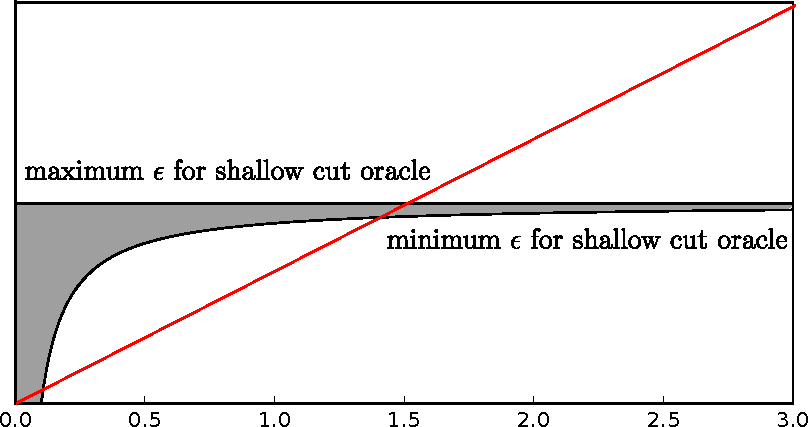
\includegraphics[width=0.65\textwidth]{cutting/epsilon_absx.pdf}
\par\end{centering}
\caption{Bounds on amount of work for shallow cut an epigraphical
cutting plane methods. The shaded gray region represents the
upper and lower bounds for the $\epsilon$ needed in the $\epsilon$-subgradient,
while the red line represents the amount of work needed in the inexact shallow
cut oracle. In epigraphical form, $\epsilon$ increases linearly with the size of the polytope.}\label{fig:bound-errors}
\end{figure} 

\end{example}

\subsection{The Maximum Inscribed Ellipsoid Oracle} 

\cite{tarasov1988method} proposed an alternate oracle as to remedy the problem
of the intractability of the center of gravity. \cite{tarasov1988method} noted
that the center of the  the maximum inscribed ellipse of a polytope shares
many of the properties of the center of gravity, but has the advantage of
being computable in polynomial time. Define an ellipse to be
$$
\mathcal{E} = \{ Ax + a\mid \|x\|\leq 1\}.
$$
Let $P$ be a convex, compact set.  Define the Maximum Inscribed Ellipsoid
(MIE) of $P$ to be ellipse of largest volume contained within $P$. For this
section only, let
$$
\mbox{\bf center}(P) := \mbox{center of MIE of $P$}.
$$
We will
also define $\volmu(P)$ to be to be the volume of this ellipse. Define, for this section only,
$$
\mbox{size}(P) = \volmu(P) = \mbox{max} \{ \vol(\mathcal{E}) \mid \mathcal{E} \mbox{ is an ellipse such that } \mathcal{E}\subseteq P \}
$$
The use of $\mbox{max}$ in place of $\sup$ is justified as the set is compact.
If 
$$P = \{ x \mid g_i^Tx \leq b_i \}$$
The MIE can be computed by solving
$$
\mbox{maximize } \log\det A \qquad \mbox{s.t.}\quad  \|Ag_i\|_2+g_i^Ta \leq b_i
$$
Like the center of gravity, a hyperplane going through the center of the MIE
divides a convex set into two approximately even parts:
\begin{thm} \label{thm:MIE_cut} \cite{tarasov1988method} 
Let $\mathcal{E}$ be the maximum volume ellipse of $P$. Then for any $g$,
$$
\frac{\volmu(P \cap \{ x \mid g^T(x - a)\leq 0\}) }{\volmu(P)} \leq 0.843  
$$
where $a$ is the center of $\mathcal{E}$.
\end{thm}

\noindent
Here we will require a slightly stronger result, Theorem $\gamma$ of
\cite{tarasov1988method}

\begin{lem} \label{lem:approx-MIE-vol} 
Let $\mathcal{E}$ be an ellipse inscribed in $P$ with relative error
$\gamma$, i.e.
$$
\vol(\mathcal{E})=(1-\gamma)\volmu(P),
$$
where $a$ is the center of this ellipse. Then
\[ 
\frac{\volmu(P\cap\{x\mid g^{T}(x-a)\leq0)}{\volmu(P)}\leq\frac{0.843}{(1-\gamma)^2}
\]
\end{lem}
\noindent Then for $P_k$'s generated by Algorithm \ref{alg:cutting_plane_epi_err},

\begin{figure}
\begin{centering}
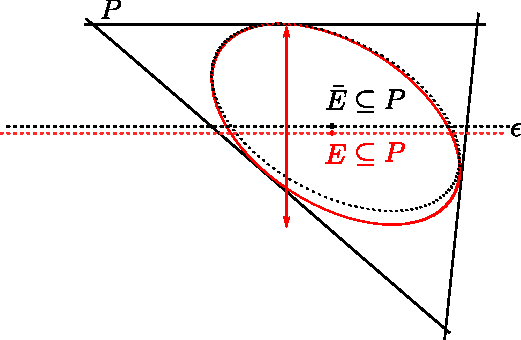
\includegraphics[width=0.65\textwidth]{cutting/fig2}
\par\end{centering}
\caption{Vertical compression of MIE to an approximate MIE}
\end{figure}

\begin{lem}\label{Rate-Decrease2}
The volumes decrease at the rate
\[
\frac{\volmu(P_{k+1})}{\volmu(P_k)}\leq\frac{0.843}{(1-\gamma)^2}
\]
\end{lem}
\begin{proof}
We will split the analysis into two cases. 

% Let $l_k$ be the linear
% lower bound given by the oarcle at iteration $k$
% \[
% l_k(x)=\inf\{t\mid(t,x)\in L_k\}=l_k+g_k^{T}(x-x_k).
% \]
% The two cases are then $l_k(x_k)\leq t_k$, and otherwise.

\noindent\textbf{Case 1: (Deep Cut) $l_k \geq t_k$ or $l_k \leq t_k$ and $u_k \leq t_k$ } 
The intersection of the cutting planes do not contain $(t_k,x_k)$, therefore by Theorem \ref{thm:MIE_cut},
\[
\frac{\volmu(P_{k+1})}{\volmu(P_k)}\leq0.843
\]
\textbf{Case 2: (Shallow Cut) $l_k < t_k$ and $u_k > t_k$}. See Figure \ref{fig:shallow-cut} for an illustration of this case. In this event, our
choice of duality gap ensures that 
\begin{equation}\label{eq:epsilon-bound}
u_k-t_k \leq u_k-l_k\leq \gamma (u^*_k - t_k) \quad \Rightarrow \quad t_k 
+ \gamma (u^*_k - t_k) \geq u_k 
\end{equation}
Consider the ellipse formed by the following compressive transformation
\begin{align*}
\bar{\mathcal{E}} & =\Lambda\left(\mathcal{E}-(u^*_k,0,\dots,0)\right)+(u^*_k,0,\dots,0)\\
\Lambda & =\mbox{diag}([1-\gamma,1,\dots,1]) 
\end{align*}
The center of this compressed ellipse is $(t_k + \gamma(u^*_k - t_k),  x_k)$
which lies at or above $(u_k,  x_k)$, by \eqref{eq:epsilon-bound}. Therefore the horizontal upper bound cuts off the center of $\bar{\mathcal{E}}$. Also observe that
$\bar{\mathcal{E}}\subseteq P$ as $P$ tapers downwards, and the vertical region that lies above  $\mathcal{E}$ is all contained in $P$. Furthermore,
\[
\vol(\bar{\mathcal{E}})=\det(\Lambda)\cdot \vol(\mathcal{E}) =(1-\gamma)\cdot\vol(\mathcal{E})
\]
Therefore, $\bar{\mathcal{E}}$ is a $(1-\gamma)$-approximate ellipsoid, and by
Lemma \ref{lem:approx-MIE-vol}
\[
\frac{\volmu(P_{k+1})}{\volmu(P_k)}\leq\frac{0.843}{(1-\gamma)^2}.
\]
Combining these two cases yields the final result.
\end{proof}
%
Applying this result inductively, we get 
$$
\volmu(P_{k})\leq\left(\frac{0.843}{(1-\gamma)^2}\right)^{k}\volmu(P_{0})
$$

Combining the above two results, we get a final theorem on the convergence rate of our algorithm.
\begin{thm}\label{thm:CG-convergence}
For all $k$ in Algorithm \ref{alg:cutting_plane_epi_err},
\[
u_{k}^{*}-f(x^{*})\leq K\left(\frac{(1-\gamma)^{2}}{0.483}\right)^{k/(n+1)}\quad K=(u_{0}-f(x^{*}))\left(\frac{\volmu(P_{0})}{\volmu(\mathcal{K})}\right)^{1/(n+1)}
\]
and therefore it terminates in no more than
\[
k = \left\lceil \frac{(n+1)\log(K/\mbox{TOL})}{-\log((1-\gamma)^2/\exp(1))} \right\rceil 
\in \mathcal{O}\left(n\log\frac{1}{\mbox{TOL}}\right).
\]
iterations with $$u^*_k - f(x^*) \leq \epsilon$$

\end{thm}

We now show a lower bound on $\epsilon_k$, an analog of Lemma \ref{lem:cg-epsilon-lower-bound}.
% We now focus our attention on the amount of work involved in each
% oracle call. Recall that the cost of invoking the oracle is inversely
% proportional to $\epsilon_k$. Hence we will show a lower bound on $\epsilon_k$
% in the next few lemmas.

% \begin{lem}
% The MIE of $P_k$ always touches the hyperplane $\{(t,x)\mid t=u^*_k\}$
% \end{lem}
% \begin{proof}
% We will show this by contradiction. Consider the case where MIE $\mathcal{E}$
% does not touch the hyperplane $\{(t,x)\mid t=u^*_k\}$. Then consider
% $\mathcal{E}$ stretched, from the bottom of the ellipsoid, till it does touch
% the hyperplane. Since $P_k$ tapers downwards, this new ellipsoid will still be
% a subset of $P$. This new Ellipse will however be strictly larger in volume
% than the original.  This is a contradiction, as  $\mathcal{E}$ is the MIE.
% \end{proof}

\begin{lem}\label{lem:mie-epsilon-lower-bound}
For all $k$,
\[
\epsilon_k\geq \frac{\gamma \, \mbox{\rm height}(P_k)}{n+1}
\]
\end{lem}
\begin{proof}
Since $u^*_k - t_k = \mbox{height}(P_k \cap \{ (t,x) \mid t \geq t_k \})$, we have from Lemma \ref{lem:MIE-1D-Div} and the definition of $\epsilon_k$
\[
\epsilon_k = \gamma \, (u^*_k - t_k) 
\geq\frac{\gamma \, \mbox{height}(P_k)}{n+1}.
\]
% \[
% f(x_k)-[\mbox{center}(\mathcal{E}_k)]_1=\mbox{height}(P\cap\{[t,0,\dots,0]\mid t\geq[\mbox{center}(\mathcal{E}_k)]_1\})
% \].
\end{proof}

Finally, we have the analog of Theorem \ref{thm:cg-total-work}. The result is
identical, apart from constants. The proof of this theorem is identical to that of Theorem $\ref{thm:cg-total-work}$.

\begin{thm}
Define the total amount of work for each oracle call $F(x,\epsilon) = \epsilon^{-1}$. Assume the algorithm is run till termination. Then the total amount of work involved is
\[
\sum{\frac{1}{\epsilon_{k}}}\leq30\cdot\frac{n+1}{\gamma \mbox{TOL}}\left\lceil (n+1)\log\left(\frac{K}{\mbox{TOL}}\right)\right\rceil \in\mathcal{O}\left(\frac{1}{\mbox{TOL}}\log\frac{1}{\mbox{TOL}}\right)
\]
\end{thm}
\begin{proof} From the bound on the total number of iterations, we get
\[
\sum {\frac{1}{\epsilon_k}} 
\leq \frac{n+1}{\gamma\mbox{TOL}}
\left\lceil \frac{(n+1)\log(K/\mbox{TOL})}{-\log((1-\gamma)^2/\exp(1))} \right\rceil
\in \mathcal{O}\left(n\log\frac{1}{\mbox{TOL}}\right).
\]
Optimizing for $\gamma$ numerically, we find that the optimum occurs at $\gamma = 0.41$. Substituting this into the equation, we get the final result.
\end{proof}

% \begin{proof}
% The algorithm terminates when either
% $$
% \mbox{height}(P_k)\leq \epsilon \qquad \mbox{ or }\qquad\volmu(P_k)\leq(\epsilon/K)^{n+1} .
% $$
% Lemma \ref{lem:cg-epsilon-lower-bound} implies the work involved at each
% iteration will be no more than $1/(50(n+1)\epsilon)$. Theorem \ref{thm:MIE-convergence} gives a bound on the total number of iterations. Multiplying the
% two quantities proves the theorem.
% \end{proof}

\section{Strongly Convex Functions}

\begin{algorithm} 
  \SetKwInOut{Input}{input}\SetKwInOut{Output}{output}
  \SetKwProg{Fn}{function}{}{end}
  \SetAlgoNoLine
  \DontPrintSemicolon
  $P_0 = C \times {[\mbox{upper bound on $f$}, \mbox{lower bound on $f$}]}$\;
  
  \While {$\max\{ \mbox{height}(P_k), K \cdot \mbox{size}(P_k)^{1/(n+1)} \} \geq \mbox{TOL}$} {
  \nl $(t_k,x_k) \gets \mbox{\bf center}(P_k)$\;
  \nl $\epsilon_k \gets \gamma (\min \{ u_0, \dots, u_{k-1}\}-t_k )$\;
  \nl $(u_k,l_k,g_k)\gets F(x_k, \epsilon_k )$\;
  \nl $P_{k+1}\gets P_k\cap 
      \underbrace{\{(t,x)\mid t\leq u_k \}}_{\mbox{\tiny upper bound}} \cap 
      \underbrace{\{(t,x)\mid l_k+g_k^{T}(x-x_k)\leq t\}}_{\mbox{\tiny lower bound}}$\;
  \vspace{-5mm}
  \nl $k \gets k+1$  
  }
  \caption{Epigraphical Cutting Plane With Error \label{alg:strongly-convex}}
\end{algorithm}

We can modify our algorithm to exploit additional structure, if available, in the problem. Consider the regularized problem
$$
\mbox{minimize}\quad  f(x) + \tfrac{S}{2}\|x\|^2  \qquad x\in C,
$$
where $f$ is convex, real valued and has a quadratic upper bound at the optimum,
\begin{equation}\label{ass:smooth}
f(x)\leq\tfrac{L}{2}\|x-x^*\|^2+f(x^*).
\end{equation}
The extra regularization parameter allows us to generate parabolic, rather than linear lower bounds on the problem: 
\[
\mbox{for any $x,\epsilon$ } \quad (u,l,g) = F(x,\epsilon),\qquad 
 l+ g^T (\bar{x}-x) +\tfrac{S}{2}\|\bar{x}\|^2 \leq f(\bar{x}) \mbox{ for all }\bar{x}.
\]
It is a simple matter to incorporate these lower bounds in this problem, and
this results in Algorithm \eqref{alg:strongly-convex}. These two modifications will enable us to prove a stronger result on the total
work involved. Indeed, in contrast to the
$\mathcal{O}(\epsilon^{-1}\log\epsilon^{-1})$ amount of work required before,
we now require $\mathcal{O}(\epsilon^{-1})$ work. For simplicity, we will assume that \mbox{\bf{center}} is the center of the MIE, and $\mbox{size}=\mu$ though all the results here can be proven for the CG in a straightfoward manner.

Let us consider why such a regularized system might arise in practice.
First, note that any unregularized, but strongly convex problem can be written
in this form (by adding and subtracting a quadratic term). Therefore this
regularized form of the problem is merely syntactic sugar - we are really
dealing with strongly convex functions. The second assumption of smoothness
holds true if $f$ is smooth and has $L$-Lipshitz gradients. This is true, for
example, if $f$ is a dual of a strongly convex primal problem. (TODO: Try to
work in a reference to Geometric Descent, a similar algorithm which uses
parabolic lower bounds. \cite{drusvyatskiy2016optimal})

In the context of constrained optimization, the regularized problem can be
interpreted as using a squared penalty in lieu  of hard constraints, as the
next example demonstrates.
% \begin{figure}
% \noindent \rule[0.5ex]{1\columnwidth}{0.5pt}
% {Parabolic Inexact Epigraphical Cutting Plane}
% \vspace{-0.5mm}

% \noindent \rule[0.5ex]{1\columnwidth}{0.5pt}

% \begin{algorithmic}
% \State $P_0\supseteq\mbox{epi}(f + \delta_C)$
% \While {$\max\{ \mbox{height}(P_k), \mathcal{O}(1)\cdot n[L^{n}\volmu(P_{k})^2]^{1/(2+n)} \} \geq\epsilon$}
%   \State $(t_k,x_k) \gets \mbox{\bf center}(P_k)$
%   \State $\epsilon_k \gets \tfrac{1}{50}(\min \{ u_0, \dots, u_{k-1}\} - t_k)$  
%   \State $(u_k,l_k,g_k)\gets F(x_k,\epsilon_k) $
%   \State $P_{k+1}\gets P_k\cap 
%       \underbrace{\{(t,x)\mid t\leq u_k \}}_{\mbox{\tiny upper bound}} \cap 
%       \underbrace{\{(t,x)\mid l_k+g_k^{T}(x-x_k) + \tfrac{S}{2}\|x\|^2\leq t\}}_{\mbox{\tiny lower bound}}$
%   \vspace{-4mm}
%   \State $k \gets k + 1$
% \EndWhile
% \end{algorithmic}
% \noindent \rule[0.5ex]{1\columnwidth}{0.5pt}
% \caption{Inexact Epigraphical Cutting plane with parabolic cuts. }\label{alg:strongly-convex}
% \end{figure}

% \noindent \rule[0.5ex]{1\columnwidth}{1pt}
% \begin{enumerate}
%   \item $P_0\supseteq\mbox{epi}(f+\delta_{\mathcal{X}})$
%   \item While $\max\{\mbox{height}(\mathcal{E}_{k}), \mathcal{O}(1)[L^{n}\volmu(P_{k})^2]^{1/(2+n)}\} \geq \epsilon $
%   \begin{enumerate}
%     \item $\mathcal{E}_k=\mbox{maximum volume ellipsoid of \ensuremath{P_k}}$
%     \item $\mbox{center}(\mathcal{E}_k)=(t_k,x_k)$
%     \item $(L_k,U_k)=\mathbf{Oracle}(x_k,\tfrac{1}{50}\mbox{height}(\mathcal{E}_k))$
%     \item $P_{k+1}=P_k\cap U_k\cap L_k$
%   \end{enumerate}
% \end{enumerate}
% \noindent\rule[0.5ex]{1\columnwidth}{1pt}

\begin{example} As noted in the motivation of the introduction, we are interested
in duals of optimization problems with few constraints. Recall the Lagrangian
\[
\mathcal{L}(v,x) = h_0(v) + x_1h_1(v) + \cdots + x_nh_n(v).
\]
Of course, as we have shown, maximizing the variable $x$ over the set $\mathbf{R}_{+}$ will recover
the original constrained problem. Instead of doing that let us regularize
the dual variables with a quadratic term, as shown:
\[
\bar{\mathcal{L}}(x,v)=h_0(v)+x_1h_1(v) + \cdots + x_nh_n(v) - \tfrac{S}{2}\|x\|^2.
\]
Now taking infimums over $v$, we see this is exactly the regularized problem
\[
-\inf_v\bar{\mathcal{L}}(x,v) = f(x) + \tfrac{S}{2}\|x\|^2.
\]
Taking supremums instead over $x$ over $\mathcal{\bar{L}}$, we arrive at an
interpretation for the regularization. We have replaced the hard constraints
with smooth,  quadratic penalties in the objective,
\[
\sup_{x\geq0}\bar{\mathcal{L}}(x,v)=h_0(v)+ \tfrac{1}{S}\big(\max\{0,h_1 (v)^2\} + \cdots + \max\{0,h_n (v)^2\}\big).
\]
If we have upper bounds on the Lagrange multipliers (our variables $x$),
$0\leq x\leq\alpha$, then the quadratic penalties turn into huber penalties. 

% we can maximize $x$ over the
% box to obtain huber penalties on the objective: 
% \[
% \mbox{minimize}\;\; \inf_{\mathclap{0\leq x\leq\alpha}}\,\bar{\mathcal{L}}(x,v)=h_0(v)+
% \tfrac{1}{S} {\textstyle \sum}_i ^{n} \max\{0, \varphi[h_i (v)]\}
% \]
% This relaxation, 
% \[
% \psi(v)=\begin{cases}
% \tfrac{1}{2}v^{2} & |v|\leq \alpha\\
% \alpha[|v|-\tfrac{1}{2}v^{2}] & |v|>\alpha
% \end{cases}
% \]
% therefore, has an interpretation of relaxing the constraints and
% turning them into penalties.
\end{example}

\begin{lem}\label{strongly_convex_upper_bound_obj}
For all $k$,
\[
u^*_k-f(x^*)\leq\mathcal{O}(1)\cdot n[L^{n}\volmu(P_k)^2]^{1/(2+n)}.
\]
where $\mathcal{O}(1)$ is a universal constant.
\end{lem}
\begin{proof}
From Assumption \ref{ass:smooth} we have the following quadratic upper bound
on $f$, 
\[
v:=\tfrac{L}{2}\|\cdot-x^*\|^2+f(x^*),
\]
i.e. $v \geq f$. Define the two sets $\mathcal{K}_k$, $\mathcal{P}_k$ for which 
$\mathcal{K}_k \subseteq \mathcal{P}_k \subseteq P_k$,
\begin{equation*}
  \mathcal{K}_k  =\mbox{conv}\{u^*_k\times\mbox{lvl}(v,u^*_k),(f(x^*),x^*)\}.
  \quad
  \mathcal{P}_k  =\mbox{epi}(v)\cap\{(t,x)\mid t\leq u^*_k\},
\end{equation*}
Also, let $\mathcal{K}$ be a unit circular cone
\[
\mathcal{K}=\mbox{conv}\big\{\{(1,x)\mid \tfrac{1}{2}\|x\|^2\leq1\},0\big\}.
\]
% The epigraph of our upper bound
% \[
% \mbox{epi}(v-f(x^*))-x^*=\{x\mid\tfrac{1}{2}\|x\|^2\leq([u_k-f(x^*)]/L)^{1/2}\}
% \]
First note that $\mathcal{K}_k$ and $\mathcal{K}$, our standard cone, are related
by a affine transformation. This transform which first involves the translation of the tip of the cones to $(0,0)$, and then a scaling.
\begin{align}\label{eq:translate_standard_cone}
\mathcal{K} & =\Sigma^{-1}_k(\mathcal{K}_k-(f(x^*),x^*))\\
\Sigma_k & =\mbox{diag}([u_k-f(x^*),([u_k-f(x^*)]/L)^{1/2},\dots,([u_k-f(x^*)/L])^{1/2})
\end{align}
Therefore, the following chain of inequalities follow:
\begin{align*}
\volmu(P_k) & \overset{(a)}{\geq}\volmu(\mathcal{P}_k) \\
& \overset{(b)}{\geq}\volmu(\mathcal{\mathcal{K}}_k) 
 \overset{(c)}{=}\det(\Sigma_k)\volmu(\mathcal{K})  
=\volmu(\mathcal{K})[u_k-f(x^*)]^{(2+n)/2}/L^{n/2}
\end{align*}
$(a)$ comes from Assumption \eqref{ass:smooth}, which implies $P_k \subseteq \mathcal{P}_k$.
$(b)$ follows from the fact that $\mathcal{P}_k\supseteq\mathcal{K}_k$,
by construction ($\mathcal{K}_k$ is a circular cone inscribed in the parabola
$\mathcal{P}_k$.)
$(c)$ comes from translating and scaling $\mathcal{K}_k$ into the standard cone, equation \eqref{eq:translate_standard_cone},  the affine invariance of the MIE, and the affine homogeneity of $\volmu$. Taking powers of $2/(2+n)$ on both sides, we get the final result
\[
u^*_k-f(x^*)
\leq\frac{L^{n/(2+n)} \volmu(P_k)^{2/(2+n)}}{\volmu(\mathcal{K})^{2/(2+n)}}
\leq\mathcal{O}(1)\cdot n[L^n\volmu(P_k)^2]^{1/(2+n)}.
\]
For the final inequality, we use the fact that 
$$\volmu(\mathcal{K})^{2/(2+n)}\geq \frac{\omega_{n}^{2/(2+n)}}{4^{\frac{2n+2}{2+n}}}\geq n \mathcal{O}(1)$$ 
for all $n$.
\end{proof}

This theorem can be seen as a quadratic improvement over Lemma
\ref{lem:lem-voldecrease}. In Lemma
\ref{lem:lem-voldecrease} we proved $ u^*_k-f(x^*)
\lessapprox \volmu(P_k)^{1/(n+1)}. $ This theorem improves that bound to $
u^*_k-f(x^*) \lessapprox \volmu(P_k)^{2/(2+n)}. $ This fact allows us to relax the
termination condition by a squared factor.  Note too, that this improvement
does not depend on the parabolic cutting  planes, and hence can be integrated
with the results in the previous section. This results in 

\begin{thm}\label{thm:MIE-convergence-2}
% For all $k$
% \[
% u^*_k-f(x^*)\leq (0.878)^{k/(n+1)}\cdot K\volmu(P_0)^{1/(n+1)}
% \]
% and when 
Algorithm \ref{alg:cutting_plane_epi_err} terminates in no more than
\[
k = \left\lceil \frac{(2+n)\log(1/\epsilon)+2\log\volmu(P_{0})+n\log L}{\log(1/0.878^{2})} \right\rceil
\in \mathcal{O}\left(n\log\frac{1}{\epsilon}\right)
\]
iterations. When Algorithm \ref{alg:strongly-convex} terminates,
\[
u^*_k - f(x^*) \leq \epsilon
\]
\end{thm}

The improvement above is not significant, and does not change the algorithms
complexity class. The above statement merely establishes that this new
stopping criteria is valid. The next theorem establishes a lower bound on
$\epsilon_k$ as a function of $\volmu(P_k)$. The parabolic lower bounds,
intuitively, prevent $P_k$ from becoming too flat.

\begin{figure}
\begin{centering}
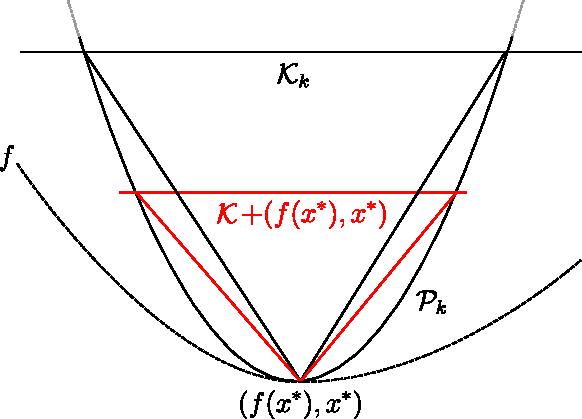
\includegraphics[width=0.65\textwidth]{cutting/fig5}
\par\end{centering}
\caption{Illustration of inner approximating cones, and the rescaling by $\Sigma_k$ necessary to transform it into the unit cone.}
\end{figure}

\begin{lem}\label{lem:strongly_convex_lower_bound_k}
For all $k$
\[
\epsilon_k\geq\mathcal{O}(1)\cdot[S{}^{n}\volmu(P_k)^2]^{1/(2+n)}
\]
Where $\mathcal{O}(1)$ is a universal constant.
\end{lem}
\begin{proof}
Let $l^*_k$ be the strongest lower bound at iteration $k$,
\[
l^*_k = \max_{i < k}\{l_i + g_i^T(\cdot-x_i) + \tfrac{S}{2}\|\cdot \|^2\}.
\]
Since each function within the $\max$ is strongly convex with modulus $S$,
so must $l^*_k$ (strong convexity is preserved by the $\max$). Let $\hat{x}^*$ be the minimizer of $l^*_k$. Since $0\in\partial l^*_k(\hat{x}^*)$ (see Figure \ref{fig:parabolic_outer_approximation}),
\[
l^*_k(x)\geq l^*_k(\hat{x}^*)+0^{T}(x-\hat{x}^*)+\tfrac{S}{2}\|x-\hat{x}^*\|^2\geq l^*_k(\hat{x}^*)+\tfrac{S}{2}\|x-\hat{x}^*\|^2,
\]
This implies $\mbox{epi}(l^*_k) \subseteq\mbox{epi}(l^*_k(\hat{x}^*)+\tfrac{S}{2}\|\cdot-\hat{x}^*\|^2)$ and therefore
\begin{align}\label{eq:subset_P_k_Parabola_k}
P_k & =\mbox{epi}(l^*_k) \cap \{(t,x) \mid t \leq u^*_k \} \\
    & \subseteq\mbox{epi}(l^*_k(\hat{x}^*)+\tfrac{S}{2}\|\cdot-\hat{x}^*\|^2)\cap \{(t,x) \mid t \leq u^*_k \}  =:\mathcal{P}_k
\end{align}
See Figure \ref{fig:parabolic_outer_approximation} for an illustration. Lete $\omega_n$ be the volume of a unit $n$-ball.
\begin{align*}
\volmu(P_k) & \overset{(a)}{\leq}\vol(P_k)\\
 & \overset{(b)}{\leq}\vol(\mathcal{P}_k) \\
 & \overset{(c)}{=}\frac{2\omega_n}{n[S/2]^{n/2}}\cdot \mbox{height}(\mathcal{P}_k)^{(2+n)/2} \\
 & \overset{(d)}{=}\frac{2\omega_n}{n[S/2]^{n/2}}\cdot \mbox{height}(P_k)^{(2+n)/2} \\
 & \overset{(e)}{\leq}\frac{2\omega_n }{n[S/2]^{n/2}} \cdot [(n+1)\epsilon_k]^{(2+n)/2}
\end{align*}
$(a)$ comes from the fact that $\volmu(P_k)=\vol(\mathcal{E}_k),$
and $\mathcal{E}_k$, being an inscribed ellipse, is a subset of
$P_k$. $(b)$ comes from \eqref{eq:subset_P_k_Parabola_k}. Finally, $(c)$ is the volume
of a parabola. $(c)$ is from construction (see Figure \ref{fig:parabolic_outer_approximation}), and $(d)$ comes from Lemma \ref{lem:MIE-1D-Div}. Taking powers of
$2/(2+n)$ on both sides, we obtain
% \[
% \epsilon_k\geq\frac{[S/2]^{n/(2+n)}}{(n+1)[n\omega_n]{}^{2/(2+n)}}\cdot\volmu(P_k)^{2/(2+n)}\geq\mathcal{O}(1)\cdot[S{}^{n}\volmu(P_k)^2]^{1/(2+n)}
% \]
\[
\epsilon_k \geq \frac{n^{2/(2+n)}}{2}\cdot \frac{[\volmu(P_{k})^{2}S^{n}]^{1/(2+n)}}{(n+1)[\omega_{n}]^{2/(2+n)}}
\geq \mathcal{O}(1)\cdot[S{}^{n}\volmu(P_k)^2]^{1/(2+n)}
\]
The final inequality comes from the Lemma \ref{vol-sphere-bound}.
% (i haven't proved the last part formally, 
% but an informal proof goes along the lines of $\omega_n^{-2/(2+n)} \in \mathcal{O}(n)$
% and so the terms should multiply to give a constant. The quantity above seems to be bounded by 18. This conjecture holds in wolfram alpha too.)
% type {\tt plot (pi^(n/2)/gamma(n/2+1))^(-2/(2+n)) for  0< n < 100} and {\tt plot (n+1)*(pi^(n/2)/gamma(1+n/2))^(2/(n+2)) for 0 < n < 300)} into wolfram alpha for plots)
\end{proof}

\begin{figure}
\begin{centering}
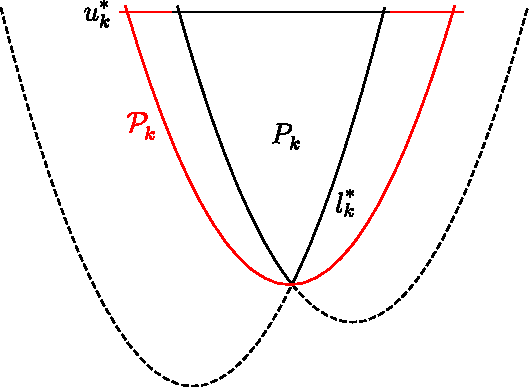
\includegraphics[width=0.65\textwidth]{cutting/fig4}
\par\end{centering}
\caption{Geometric Illustration of the parabolic outer approximation
of $P_k$, i.e. $P_k \subseteq \mathcal{P}_k$. \label{fig:parabolic_outer_approximation}}
\end{figure}


Finally, we bound the total amount of work involved in the algorithm. We assume that the amount of work is inversely proportional to $\epsilon$. 

\begin{thm}
Assume the algorithm is run till termination. Then for $\epsilon>0$
\[
\sum\frac{1}{\epsilon_k}\leq\frac{L}{S}\cdot\frac{\mathcal{O}(1)}{1-0.878^{2/(2+n)}}\cdot\frac{n}{\epsilon}
\]
Where $\mathcal{O}(1)$ represents a universal constant.
\end{thm}
\begin{proof}
Let $\volmu_k:=\volmu(P_k)^{2/(2+n)}.$ Then we have the following three
guarantees. 
\begin{alignat*}{2}
  \epsilon_k & \geq C_1\volmu_k &  & \mbox{(Lower bound on $\epsilon_k$, Lemma \ref{lem:strongly_convex_lower_bound_k})}\\
  \volmu_k & \geq C_2\epsilon & \qquad & \mbox{(Termination criteria, Algorithm \ref{alg:strongly-convex})}\\
  \volmu_k & \geq0.878^{-2/(2+n)}\cdot\volmu_{k+1} &  & \mbox{(Convergence guarantee, Lemma \ref{Rate-Decrease2})}
\end{alignat*}
where
\[
C_1=\mathcal{O}(1)\cdot S^{n/(2+n)},\qquad C_2=\mathcal{O}(1)\cdot L^{-n/(2+n)}
\]
Therefore, the total cost of the iteration is 
\[
\sum\frac{1}{\epsilon_k}\leq\sup\{\alpha_0,\alpha_1,\dots\},
\]
where $\alpha_j$ is the total amount of work performed if the algorithm
ran for $j$ steps. We can upper bound the total amount of work performed 
by performing an optimization over the three constraints described above.
Let $\beta=0.878^{-2/(2+n)}.$ Then 
\begin{align*}
\alpha_{j} 
  & \leq \sup\,\{\,{\textstyle \sum_{k=0}^j}\epsilon_k^{-1}\mid\volmu_0\geq\beta\volmu_1,\cdots,\volmu_{j-1}\geq\beta\volmu_{j}\mbox{ and }\volmu_k\geq C_2\epsilon,\epsilon_k\geq C_1\volmu_k\mbox{, $\forall k$}\}\\
  & =\sup\,\{\,{\textstyle \sum_{k=0}^j}\,\epsilon_k^{-1}\mid\volmu_0\geq\beta\volmu_1,\cdots,\volmu_{j-1}\geq\beta\volmu_{j}\mbox{ and }\volmu_k\geq C_2\epsilon,\epsilon_k=C_1\volmu_k\mbox{, $\forall k$}\}\\
  & =\sup\,\{\,{\textstyle \sum_{k=0}^j}\,[C_1\volmu_k]^{-1}\mid\volmu_0\geq\beta\volmu_1,\cdots,\volmu_{j-1}\geq\beta\volmu_{j},\volmu_j\geq C_2\epsilon\}\\
  & \overset{(1)}{=}\frac{{\textstyle \sum_{k=0}^j}\beta^{-k}}{C_1C_2\epsilon}
  \leq \frac{{\textstyle \sum_{k=0}^{\infty}}\beta^{-k} } { C_1C_2\epsilon}
  =\frac{1}{( 1-{\beta^{-1}} )C_1C_2\epsilon } 
\end{align*}
Inequality $(1)$ comes from Lemma \ref{lem:maximization_convex}. Our objective function
is convex, and bounded from above on the feasible set (the function is decreasing, and the feasible set does not contain $0$). By writing the constraints as
$$ 
\left(\begin{array}{cccc}
1 & -\beta\\
 & \ddots & \ddots\\
 &  & 1 & -\beta\\
 &  &  & 1
\end{array}\right)\left(\begin{array}{c}
\volmu_{0}\\
\vdots\\
\volmu_{j-1}\\
\volmu_{j}
\end{array}\right)\geq\left(\begin{array}{c}
0\\
\vdots\\
0\\
C_2\epsilon
\end{array}\right).
$$
The statement of the lemma states that the optimum is achieved at equality. Therefore the optimum is achieved at $\volmu_{k}=\beta^{j-k}C_2\epsilon$. Substituting this back into the objective and reversing the order of summation yields the equality. Finally,
\[
\frac{1}{C_1C_2}=
\frac{\mathcal{O}(1)\cdot n L^{n/(2+n)}}{\mathcal{O}(1)\cdot S^{n/(2+n)}} 
\leq\mathcal{O}(1)\cdot\frac{n L}{S}
\]
as $L/S \geq 1$ which implies $(L/S)^p
\leq L/S$ for $p\leq1$
\end{proof}
%

Surprisingly, there are no constants in the above proof which involve
$\volmu(P_0)$. This counterintuitive fact means the volume of the initial
localization polytope plays no role in the optimization. How can this be
possible?  Perhaps this can be understood with the following intuition. Since
the iterates at the beginning get exponentially cheaper as the polytope $P_0$
increases, in a sense, early iterations contribute very little to the work
involved. In practice, of course, this is not the case. There is some, finite
fixed cost in solving any optimization problem, which cannot be atomically
divided. However we believe that this property still translates to much better
performance in practice.

\section{Some General Facts}
\begin{lem} \label{vol-paranolid}
({\bf Volume of a Parabolid}) Let $\omega_n$ be the volume of the $n$ unit ball. Then
\[
{\rm vol}(\{(t,x)\mid\tfrac{K}{2}\|x\|^2\leq t \leq h\})=
\frac{2\omega_n}{n[K/2]^{n/2}}\cdot h^{(2+n)/2}.
\]
\end{lem}
\begin{proof}
This proof is an application of the ``disk method'' in calculus.
Since
\[
\frac{K}{2}\|x\|^2\leq t\iff\|x\|\leq\sqrt{2t/K},
\]
each slice of $\mathcal{P}$ in the first dimension is a $n-$ball
of radius $\sqrt{2t/K}$, with area $\omega_n(2t/K)^{n/2}$. We integrate
this from $0$ to $h$,
i.e.,
\[
{\rm vol}(\mathcal{P})=
\omega_n\int_0^{h}[2t/K]{}^{n/2}dt=
\frac{\omega_n}{[K/2]^{n/2}}\int_0^{h}t^{n/2}dt=
\frac{2\omega_n}{n[K/2]^{n/2}}\cdot h^{(n+2)/2}.
\]
\end{proof}
%

\begin{lem} (Volume approximations for MIE of the unit circular cone)
Let 
$$\mathcal{K} = \mbox{\normalfont conv}\big\{\{(1,x)\mid \tfrac{1}{2}\|x\|^2\leq1\},0\big\}.$$ Then $$ \frac{\omega_{n+1}}{4^{n+1}} \leq \volmu({\mathcal{K}}) \leq \frac{2^{n/2+1}\omega_{n}}{n}$$
\end{lem}
\begin{proof} {(\bf{Lower Bound})} We can inscribe a $n+1$ dimensional ball of radius $1/(2\sqrt{1.25} + 1)$ in the unit cone. Since the MIE is larger than this,
$$\frac{\omega_{n+1}}{(2\sqrt{1.25}+1)^{n+1}} \leq \volmu(\mathcal{K}).$$
{(\bf{Upper Bound})} Since $\volmu(\mathcal{K}) \leq \mbox{vol}(\mathcal{K})$, we can use Lemma \ref{vol-paranolid}
\end{proof}

\begin{lem}\label{lem:maximization_convex}
({\bf Maximization of a convex function over a cone}) Let $f$ be
a convex function, and $A$ be a square, invertible matrix. Furthermore assume that $f$ is bounded on the
cone $\{x\mid Ax\geq b\}$. Then 
\[
\sup_{x}\,\{f(x)\mid Ax\geq b\} = f(A^{-1}b).
\]
\end{lem}
\begin{proof}
We transform the problem to 
\[
\sup_{x}\,\{f(x)\mid Ax\geq b\}=\sup_{x}\,\{f(A^{-1}(x+b))\mid x\geq0\}=\sup_{x}\{g(x)\mid x\geq0\}
\]
Where $g(x)=f(A^{-1}(x+b))$. By assumption, the function $g$ is bounded, and
therefore is decreasing on every half line \cite{Roc70}, and achieves the
maximum at $g(0)$. Therefore, $g$ must attain a global minimum at $g(0)=f(A^{-1}b)$.
\end{proof}

\begin{lem}\label{lem:MIE-1D-Div}
Let $P\subseteq R^{n+1}$ be a compact polytope, and assume that the
center of the maximum volume elipsoid of $P$ is $a$. Then
\[ 
\frac{1}{n+1}\leq
\frac{\mbox{\rm height}
(\ensuremath{P\cap \{(t,x)\mid t\geq a_1\})}}{\mbox{\rm height(\ensuremath{P})}}
\leq\frac{n}{n+1}
\]
\end{lem}
\begin{proof}
Let $\mathcal{E}$ be the MIE of $P$. Assume, w.l.o.g, $\mathcal{E}$ is centered at $0$. By \cite{tarasov1988method} we know that
\[
\mathcal{E}\subseteq P\subseteq n \mathcal{E}
\]
Define the $\mbox{Proj}$ to be the projection of the set $P$ onto
the first coordinate,
\[
\mbox{Proj}(P)=\{t\mid(t,\bar{x})\in P\mbox{\}}
\]
Since $\mathcal{E},P,n \mathcal{E}$ are all convex, their corrosponding projections are
intervals. Since $\mathcal{E},n \mathcal{E}$ are both ellipses centered at $0$, we can
assume then without loss of generality (since the ratios are preserved)
\[
\mbox{Proj}(\mathcal{E}):=[-1,1],\quad\mbox{Proj}(P):=[-x_1,x_2],\quad\mbox{Proj}(n \mathcal{E}):=[-n,n]
\]
Using the fact that 
\[
\mbox{Proj}(\mathcal{E})\subseteq\mbox{Proj}(P)\subseteq\mbox{Proj}(n \mathcal{E})
\]
we have
\[
[-1,1]\subseteq[-x_1,x_2]\subseteq[-n,n]
\]
Then for $H = \{(t,x)\mid t\geq a_1\})$
\[
\frac{\mbox{height(\ensuremath{P\cap H)} }}{\mbox{height(\ensuremath{P})}}=\frac{x_1}{x_2+x_1}\leq\sup\left\{ \frac{x_1}{x_2+x_1}\,\Big|\;\begin{array}{c}
1\leq x_1\leq n\\
1\leq x_2\leq n
\end{array}\right\} =\frac{n}{n+1}
\]
The final equality can be found by solving a simple $2d$ optimization
problem over a box, for which we can exhaustively search all critical
points. Replacing the $\sup$ with an $\inf$, we obtain the other bound.
\end{proof}

\begin{figure}
\begin{centering}
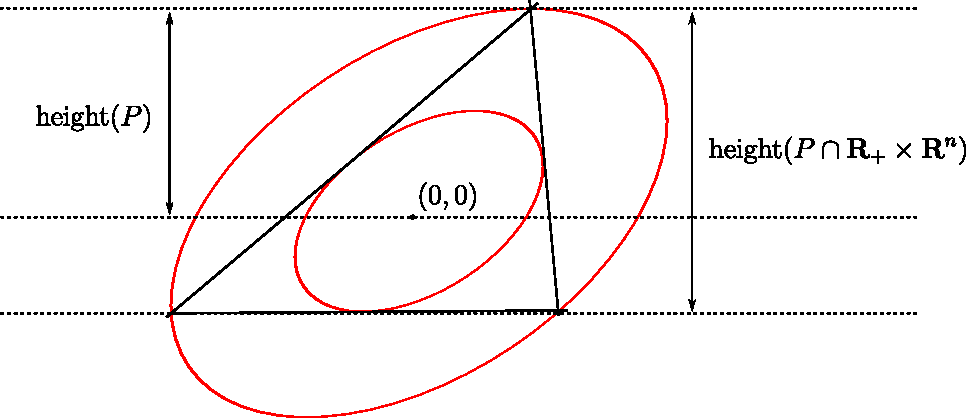
\includegraphics[width=0.65\textwidth]{cutting/fig1}
\par\end{centering}
\caption{Case where lower bound is tight in $2d$. The $n-$dimensional simplex
achieves this bound in general.}

\end{figure}

\begin{lem} \label{vol-sphere-bound}
Let $\omega_n$ be the volume of a unit sphere. Then

$$ \frac{2}{n+1} \leq \omega_{n}^{2/(2+n)}\leq \frac{12}{n+1}$$
\end{lem}
\begin{proof} Multiplying both sides by $n+1$, we get
\begin{align*}
(n+1)\omega_{n}^{2/(2+n)} & =(n+1)\left(\frac{\pi^{\frac{n}{2}}}{\Gamma(\frac{n}{2}+1)}\right)^{2/(2+n)}\\
 & \overset{(a)}{\leq}(n+1)\left(\frac{\pi^{\frac{n}{2}}}{\sqrt{2\pi}n^{\frac{n+3}{2}}e^{-\frac{n+2}{2}}}\right)^{2/(2+n)}\\
 & =(n+1)\frac{\pi^{\frac{n}{2+n}}}{\sqrt{2\pi}n^{\frac{n+3}{n+2}}e^{-1}}\\
 & =\frac{n+1}{n^{1+\frac{1}{n+2}}}\frac{\pi^{\frac{n}{2+n}}}{\sqrt{2\pi}e^{-1}}\\
 & \leq\left(1+\frac{1}{n}\right)\frac{3\pi e}{\sqrt{2\pi}}
  \leq\frac{6\pi e}{\sqrt{2\pi}} \leq 12
\end{align*}
$(a)$ comes from sterling's lower bound. The lower bound is proved in an analogous way
\begin{align*}
(n+1)\omega_{n}^{2/(2+n)} & =(n+1)\left(\frac{\pi^{\frac{n}{2}}}{\Gamma(\frac{n}{2}+1)}\right)^{2/(2+n)}\\
 & \geq(n+1)\left(\frac{\pi^{\frac{n}{2}}}{\sqrt{2\pi}\cdot n^{n+\frac{1}{2}}e^{\frac{1}{12n}-n}}\right)^{2/(2+n)}\\
 & =(n+1)\frac{\pi^{\frac{n}{2+n}}}{\sqrt{2\pi}\cdot n^{\frac{n+3}{2+n}}e^{\left(\frac{2}{2+n}\right)\left(\frac{1}{12n}-n\right)}}\\
 & \geq\frac{n+1}{n}\frac{10}{\sqrt{2\pi}}
\end{align*}
\end{proof}
